%!TEX root = ../Osteuropaatlas.tex


\section{Bruttoinlandsprodukt \& Bruttowertschöpfung}

\begin{table}[!h]
	\addcontentsline{toc}{subsection}{Wechselkurse Osteuropäischer Währungen}
	\caption{Wechselkurse Osteuropäischer Währungen}
	\begin{tblr}{
			width = \linewidth,
			rowsep = 1pt,
			colspec = {|X[1.5,c,m]|X[r,m]|X[r,m]|X[r,m]|X[r,m]|X[r,m]|},
			row{odd} = {bg=imreg!20},
			row{1} = {c,bg=imreg,fg=white,font=\bfseries\large, rowsep=8pt},
			cell{3}{4} = {c}
		}
		\hline
		Wechselkurse & 2010 & 2015 & 2023 & $\Delta$ 2023/2010 & $\Delta$ 2023/2015 \\
		\hline
		{Bulgarischer Lew\\(BGN / EUR)} & 1,96 & 1,96 & 1,96 & ±0,0\% & ±0,0\% \\
		\hline
		{Kroatische Kuna\\(HRK / EUR)} & 7,29 & 7,61 & {\euro{} seit 2023} &  &  \\
		\hline
		{Polnischer Zloty\\(PLN / EUR)} & 3,99 & 4,18 & 4,54 & +13,78\% & +8,61\% \\
		\hline
		{Rumänischer Leu\\(RON / EUR)} & 4,21 & 4,45 & 4,95 & +18\% & +11,24\% \\
		\hline
		{Tschechische Krone\\(CZK / EUR)} & 25,28 & 27,28 & 24,00 & -5,06\% & -12,02\% \\
		\hline
		{Ungarischer Forint\\(HUF / EUR)} & 275,48 & 310 & 381,76 & +38,58\% & +23,15\% \\
		\hline
	\end{tblr}
	\begin{spacing}{1} \scriptsize
		\vspace{2mm}
		Anm.: Jahresdurchschnitte; Stand 2023\\
		Quelle: Deutsche Bundesbank (2024); Ber. imreg (2024) \end{spacing}
\end{table}


\setcounter{figure}{0}
\begin{figure}[!h]
	\addcontentsline{toc}{subsection}{Wechselkursindex}
	\caption{Wechselkursindex}
	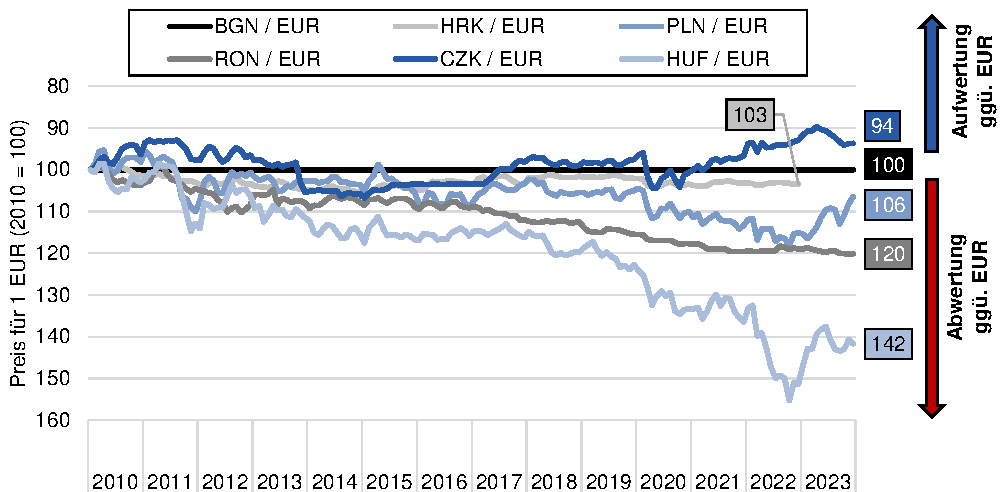
\includegraphics[width = \textwidth, height = 8.33cm]{Wechselkurse}
	\begin{spacing}{1} \scriptsize
		\vspace{2mm}
		Anm.: Indexwert 2010 = 100; Stand 2023\\
		Quelle: Deutsche Bundesbank (2024); Ber. imreg (2024) \end{spacing}
\end{figure}



\begin{figure}[p]
	\addcontentsline{toc}{subsection}{Bruttoinlandsprodukt (in realen Preisen)}
	{\centering \maps{Bruttoinlandsprodukt (in realen Preisen)}}
	\label{map:bip}
	\karte{BIP}{2021}{Veränderung 2015 bis 2021}
	\begin{spacing}{1} \scriptsize
		Anm.: Stand 2021\\
		Quelle: Eurostat (2024); Ber. \& Dar. imreg (2024) \end{spacing}
\end{figure}


\begin{figure}[p]
	\addcontentsline{toc}{subsection}{Bruttoinlandsprodukt je Einwohner}
	{\centering \maps{Bruttoinlandsprodukt je Einwohner}}
	\label{map:bippc}
	\karte{BIP_proKopf}{2021}{Veränderung 2015 bis 2021}
	\begin{spacing}{1} \scriptsize
		Anm.: Stand 2021\\
		Quelle: Eurostat (2024); Ber. \& Dar. imreg (2024) \end{spacing}
\end{figure}


\begin{figure}[p]
	\addcontentsline{toc}{subsection}{Bruttoinlandsprodukt (in Kaufkraftstandards)}
	{\centering \maps{Bruttoinlandsprodukt (in Kaufkraftstandards)}}
	\label{map:bipkks}
	\karte{BIP_KKS}{2021}{Veränderung 2015 bis 2021}
	\begin{spacing}{1} \scriptsize
		Anm.: KKS = Kaufkraftstandards; Stand 2021\\
		Quelle: Eurostat (2024); Ber. \& Dar. imreg (2024) \end{spacing}
\end{figure}


\begin{figure}[p]
	\addcontentsline{toc}{subsection}{Bruttoinlandsprodukt je Einwohner (in Kaufkraftstandards)}
	{\centering \maps{Bruttoinlandsprodukt je Einwohner (in Kaufkraftstandards)}}
	\label{map:bipkkspc}
	\karte{BIP_KKS_proKopf}{2021}{Veränderung 2015 bis 2021}
	\begin{spacing}{1} \scriptsize
		Anm.: KKS = Kaufkraftstandards, Stand 2021\\
		Quelle: Eurostat (2024); Ber. \& Dar. imreg (2024) \end{spacing}
\end{figure}


\begin{figure}[p]
	\addcontentsline{toc}{subsection}{Entwicklung Volumenindex}
	{\centering \maps{Entwicklung Volumenindex}}
	\label{map:bipvolidx}
		\makebox[\linewidth][c]{
		\begin{subfigure}{0.61\textwidth}
			\centering
			\caption{Volumenindex Bruttoindlandsprodukt\\Veränderung 2015 bis 2021}
			\includegraphics[width=\textwidth, height=172mm, center]{BIP_Vol_Delta} 
		\end{subfigure}
		\begin{subfigure}{0.61\textwidth}
			\centering
			\caption{Volumenindex Bruttowertschöpfung\\Veränderung 2015 bis 2021}
			\includegraphics[width=\textwidth, height=172mm, center]{BWS_Vol_Delta}
		\end{subfigure}
	}
	\begin{spacing}{1} \scriptsize
		Anm.: Veränderungen relativ zum EU-27-Mittel; Stand 2021\\
		Quelle: Eurostat (2024); Ber. \& Dar. imreg (2024) \end{spacing}
\end{figure}



